\documentclass[aspectratio=1610,12pt]{beamer}
\usepackage{tikz-cd}
\usepackage{ebproof}
\usepackage{booktabs}
\usetikzlibrary{patterns}

\newcommand{\que}{\circ}
\newcommand{\ans}{\bullet}

\begin{document}

\section{Compositionality in CompCert}
\frame{\sectionpage}

\begin{frame}{Semantics in CompCert} %{{{
  CompCert's correctness is established using a simulation:
  \begin{equation}
    \mathsf{CompCert}(p) = p' \quad\Longrightarrow\quad
    \mathsf{Clight}(p) \:\le\: \mathsf{Asm}(p') %\:\in\: \mathsf{TS}
    \label{eqn:compcertcorrect}
  \end{equation}

  \vfill
  For each source, target and intermediate program $p \in L$, \\
  a transition system
  $L(p) = \langle S, {\rightarrow}, I, F \rangle$ is defined where:
  \[
    S \in \mathbf{Set} \qquad
    {\rightarrow} \subseteq S \times S \qquad
    I \subseteq S \qquad
    F \subseteq S \times \mathsf{int}
  \]
  An execution of $p$ corresponds to a transition sequence:
  \[
    I \ni s_0 \rightarrow s_1 \rightarrow \cdots \rightarrow s_n \mathrel{F} x
  \]

  \vfill
  Simulations prove the correctness of each pass,
  and are composed to derive (\ref{eqn:compcertcorrect}).
\end{frame}
%}}}

\begin{frame}[fragile]{Simulations} %{{{
  %CompCert is broken down in compilation phases
  %which are verified individually.

  %\vfill
  A simulation $\rho : L_1 \le L_2 \in \mathsf{TS}$ of $L_1$ by $L_2$
  is a relation $\rho \subseteq S_1 \times S_2$ such that:
  \vspace{-1ex}
  \begin{columns}
    \begin{column}{.68\textwidth}
      \begin{itemize}
        \item $s_1 \in I_1 \:\Rightarrow\: \exists s_2 \mathbin.
          s_2 \in I_2 \:\wedge\: s_1 \mathrel{\rho} s_2$
        \item $s_1 \mathrel{\rho} s_2 \:\wedge\: s_1 \rightarrow_1 s_1'
          \:\Rightarrow\: \exists s_2' \mathbin.
            s_2 \rightarrow_2 s_2' \:\wedge\: s_1' \mathrel{\rho} s_2'$
        \item $s_1 \mathrel{\rho} s_2 \:\wedge\: s_1 \mathrel{F_1} x
          \:\Rightarrow\: s_2 \mathrel{F_2} x$,
      \end{itemize}
    \end{column}
    \begin{column}{.25\textwidth}
      \[
      \begin{tikzcd}
        s_1 \ar[d,"\rho"',dash] \ar[r] & s_1' \ar[d,dashed,dash,"\rho"] \\
        s_2 \ar[r,dashed] & s_2'
      \end{tikzcd}
      \]
    \end{column}
  \end{columns}
  \vspace{1ex}
  so that any execution of $L_1$ yields a
  a similar execution of $L_2$.

  \begin{columns}
    \begin{column}{.68\textwidth}
  Simulation relations compose in the expected way:
  \[
    \begin{prooftree}
      \hypo{\rho : L_1 \le L_2}
      \hypo{\pi : L_2 \le L_3}
      \infer2{(\rho \mathbin; \pi) : L_1 \le L_3}
    \end{prooftree}
  \]
  making it possible to decompose the correctness proof.
    \end{column}
    \begin{column}{.25\textwidth}
      \[
        \begin{tikzcd}[column sep=0.5ex]
          L_1 \ar[d, Rightarrow, "\rho"] &&
          L_1 \ar[dd, Rightarrow, "\rho \mathbin; \pi"] \\
          L_2 \ar[d, Rightarrow, "\pi"] & \vdash \\
          L_3 && L_3
        \end{tikzcd}
      \]
    \end{column}
  \end{columns}
\end{frame}
%}}}

\begin{frame}{Vertical Composition \fbox{$;$}} %{{{
  In other words, transition systems and simulations form a category:
  \begin{itemize}
    \item the objects are transition systems
    \item the morphisms from $L_1$ to $L_2$ are the simulations $L_1 \le L_2$
    \item The composition $;$ of simulations is associative
    \item $=$ is always a simulation relation and a unit for $;$
  \end{itemize}

  \vfill
  This can be summarized by the following ``compositionality signature'':
  \begin{center}
    \begin{tabular}{lcc}
      \toprule
      \multicolumn{3}{c}{\textbf{CompCert}} \\
      \midrule
      Object & Dimension & Operations \\
      \midrule
      Transition system & 0 \\
      Simulation & 1 & $\mathbin;$ \\
      \bottomrule
    \end{tabular}
  \end{center}
\end{frame}
%}}}

\begin{frame}{Semantics in Compositional CompCert} %{{{
  Compositional CompCert models to behavior of individual translation units.

  \vfill
  Schematically,
  transition systems are extended to
  $L = \langle S, {\rightarrow}, I, X, Y, F \rangle$
  where
  \begin{align*}
    I &\:\subseteq\: (\mathsf{ident} \times \mathsf{val}^* \times \mathsf{mem}) \times S
    &
    F &\:\subseteq\: S \times (\mathsf{val} \times \mathsf{mem})
    \\
    X &\:\subseteq\: S \times (\mathsf{ident} \times \mathsf{val}^* \times \mathsf{mem})
    &
    Y^{s_x} &\:\subseteq\: (\mathsf{val} \times \mathsf{mem}) \times S
  \end{align*}
  Then an execution handles an incoming call and
  can perform outgoing calls:
  \[
    \mathsf{enq}(\vec{v})@m
    \mathrel{I}
    s_0 \rightarrow^* s_1
    \mathrel{X}
    \mathsf{inc}(\epsilon)@m_1 \leadsto 5@m_1'
    \mathrel{Y^{s_1}}
    s_2 \rightarrow^* \cdots \rightarrow^* s_n
    \mathrel{F}
    \mathsf{undef}@m'
  \]

  \vfill
  \emph{Linking} is modeled
  by letting transition systems
  handle each others' calls.

  Formally, this takes the form of a \emph{semantic linking} operator $\oplus$:
  \[
    L_1, L_2 \in \mathbf{TS} \: \vdash \: L_1 \oplus L_2 \in \mathbf{TS}
  \]
\end{frame}
%}}}

\begin{frame}{Horizontal Composition $\oplus$} %{{{
  For this to be useful, this mode of composition must propagate to simulations:
  \[
    \begin{prooftree}
      \hypo{\rho_1 : L_1 \le L_1'}
      \hypo{\rho_2 : L_2 \le L_2'}
      \infer2{\rho_1 \oplus \rho_2 : L_1 \oplus L_2 \le L_1' \oplus L_2'}
    \end{prooftree}
  \]

  \vfill
  The corresponding composition signature is that of a \emph{monoidal category}:
  \begin{center}
    \begin{tabular}{lccc}
      \toprule
      \multicolumn{4}{c}{\textbf{Compositional CompCert}} \\
      \midrule
      Object & Dimension & \multicolumn{2}{c}{Ops} \\
      \midrule
      Transition system & 1 & & $\oplus$ \\
      Simulation & 2 & $\mathbin;$ & $\oplus$ \\
      \bottomrule
    \end{tabular}
  \end{center}
\end{frame}
%}}}

\begin{frame}[fragile]{Pasting diagrams} %{{{
\[
  \begin{tikzcd}
    L^\sharp \ar[d, "\rho", Rightarrow] \\
    L^\natural \ar[d, "\pi", Rightarrow] \\
    L^\flat
  \end{tikzcd}
  \qquad\qquad\qquad\pause
  \begin{tikzcd}[sep=tiny]
    * \ar[dd, equal] \ar[rr, "L_1^\sharp", dash] &&
    * \ar[dd, equal] \ar[rr, "L_2^\sharp", dash] &&
    * \ar[dd, equal]
    \\
    & \rho_1 & & \rho_2 &
    & \rho_1 : L_1^\sharp \le L_1^\natural
    \\
    * \ar[dd, equal] \ar[rr, "L_1^\natural"', dash] &&
    * \ar[rr, "L_2^\natural"', dash] &&
    * \ar[dd, equal]
    & \rho_2 : L_2^\sharp \le L_2^\natural
    \\
    && \pi &&
    & \pi : L_1^\natural \oplus L_2^\natural \le L^\flat
    \\
    * \ar[rrrr, "L^\flat"', dash] && &&
    *
  \end{tikzcd}
\]
\end{frame}
%}}}

\begin{frame}{String diagrams} %{{{
  A simulation $\phi : L_1 \oplus \cdots \oplus L_n \le L'_1 \oplus \cdots \oplus L'_m$
  can be depicted as:
  \[
    \includegraphics[scale=0.1]{phi}
  \]

  \vspace{-1ex}
  Diagrams of this sort compose in both directions:
  \[
    \includegraphics[scale=0.1]{composite}
  \]
\end{frame}
%}}}

\begin{frame}{Semantics in CompCertO} %{{{
  \only<1>{
    Recall the transition systems
    $L = \langle S, {\rightarrow}, I, X, Y, F \rangle \in \mathbf{TS}$
    used in CompComp:
    \begin{align*}
      I &\:\subseteq\: (\mathsf{ident} \times \mathsf{val}^* \times \mathsf{mem}) \times S
      &
      F &\:\subseteq\: S \times (\mathsf{val} \times \mathsf{mem})
      \\
      X &\:\subseteq\: S \times (\mathsf{ident} \times \mathsf{val}^* \times \mathsf{mem})
      &
      Y^{s} &\:\subseteq\: (\mathsf{val} \times \mathsf{mem}) \times S
    \end{align*}
    One challenge is that values and memory states are transformed.
  }
  \pause
  \only<2->{
  In CompCertO, we generalize
  $L = \langle S, {\rightarrow}, I, X, Y, F \rangle \in \mathbf{TS}(A)$
  to:
  \begin{align*}
    I &\:\subseteq\: A^\circ \times S
    &
    F &\:\subseteq\: S \times A^\bullet
    \\
    X &\:\subseteq\: S \times A^\circ
    &
    Y^{s} &\:\subseteq\: A^\bullet \times S
  \end{align*}
  for a \emph{language interface} $A = \langle A^\circ, A^\bullet \rangle$.
  }
  \pause\vfill
  \begin{center}
    \begin{tabular}{lccc}
      \toprule
      \multicolumn{4}{c}{\textbf{CompCertO} (so far)} \\
      \midrule
      Object & Dimension & \multicolumn{2}{c}{Ops} \\
      \midrule
      \textbf{Language interface} & 0 & \\
      Transition system & 1 & & $\oplus$ \\
      Simulation & 2 & $\mathbin;$ & $\oplus$ \\
      \bottomrule
    \end{tabular}
  \end{center}
\end{frame}
%}}}

\begin{frame}[fragile]{Simulations in CompCertO} %{{{
  To connect source and target languages such as
  \[
    \mathsf{Clight}(p) \in \mathbf{TS}(\mathcal{C})
    \qquad
    \textit{vs}
    \qquad
    \mathsf{Asm}(p') \in \mathbf{TS}(\mathcal{A})
    \,,
  \]
  we then introduce simulation \emph{conventions} $\mathbb{R} : \mathcal{C} \Leftrightarrow \mathcal{A}$,
  which parameterize \\
  the relationship between source- and target-level interactions:
  \[
    \begin{tikzcd}
      \mathcal{C}^\circ \ni {} \hspace{-3em} &
      q_1 \ar[r, dash, "I_1"] \ar[d, "\mathbb{R}^\circ"', dash] & s_1 \ar[d, "\rho", dash, dashed] &
      s_1 \ar[r] \ar[d, dash, "\rho"'] & s_1' \ar[d, dashed, dash, "\rho"] &
      s_1 \ar[r, dash, "F_1"] \ar[d, dash, "\rho"'] & r_1 \ar[d, "\mathbb{R}^\bullet", dashed, dash]
      & \hspace{-3em} {} \in \mathcal{C}^\bullet
      \\
      \mathcal{A}^\circ \ni {} \hspace{-3em} &
      q_2 \ar[r, dash, dashed, "I_2"'] & s_2 &
      s_2 \ar[r, dashed] & s_2' & s_2 \ar[r, dashed, dash, "F_2"] & r_2
      & \hspace{-3em} {} \in \mathcal{A}^\bullet
    \end{tikzcd}
  \]
  We can now account for memory transformations and
  the relationship between C calls and their assembly-level representation.
\end{frame}
%}}}

\begin{frame}{Composition in CompCertO} %{{{
  Simulation conventions must be take into sccount in the compositional structure:
  \[
    \begin{prooftree}
      \hypo{\rho : L_1 \le_\mathbb{R} L_2}
      \hypo{\pi : L_2 \le_\mathbb{S} L_3}
      \infer2{(\rho \mathbin; \pi) : L_1 \le_\mathbb{R \mathbin; S} L_3}
    \end{prooftree}
    \qquad
    \begin{prooftree}
      \hypo{\rho : L_1 \le_\mathbb{R} L_1'}
      \hypo{\pi : L_2 \le_\mathbb{R} L_2'}
      \infer2{\rho \oplus_\mathbb{R} \pi \: : \: L_1 \oplus_A L_2 \: \le_\mathbb{R} \: L_1' \oplus_B L_2'}
    \end{prooftree}
  \]
  \vfill
  Attempting to sum up with some degree of precision:
  \begin{center}
    \begin{tabular}{llcll}
      \toprule
      \multicolumn{5}{c}{\textbf{CompCertO} (so far)} \\
      \midrule
      Object & & Dimension & \multicolumn{2}{c}{Operations} \\
      \midrule
      \textbf{Language interface} & $A$ & 0 & \\
      Transition system & $L \in \mathbf{TS}(A)$ & 1 & & $\oplus_A$ \\
      \textbf{Simulation convention} & $\mathbb{R} : A \Leftrightarrow B$ & 1 & $\mathbin;_{A,B,C}$ \\
      Simulation & $\rho : L_1 \le_\mathbb{R} L_2$ & 2 & $\mathbin;_{A,B,C,\mathbb{R,S}}$ & $\oplus_{A,\mathbb{R}}$ \\
      \bottomrule
    \end{tabular}
  \end{center}
\end{frame}
%}}}

\begin{frame}[fragile]{Incoming vs. Outgoing Calls in CompCertO} %{{{
  Unfortuntely, existing CompCert correctness proofs establish
  \begin{itemize}
    \item weaker guarantees for their \emph{incoming} calls
    \item than they rely on for their \emph{outgoing} calls.
  \end{itemize}

  \vfill
  So we must evolve our framework again, so that
\begin{columns}
  \begin{column}{.55\textwidth}
    \begin{itemize}
      \item transition systems $L : A \twoheadrightarrow B$ and
      \item simulations $\rho : L_1 \le_{\mathbb{R} \twoheadrightarrow \mathbb{S}} L_2$
    \end{itemize}
    now decouple
    \begin{itemize}
      \item the outgoing language interface $A$ \\ and simulation convention $\mathbb{R}$ from
      \item the incoming language interface $B$ \\ and simulation convention $\mathbb{S}$
    \end{itemize}
  \end{column}
  \begin{column}{.4\textwidth}
    \[
      \begin{tikzcd}
        A_1 \ar[rr, twoheadrightarrow, "L_1"] \ar[dd, Leftrightarrow, "\mathbb{R}"'] && B_1 \ar[dd, Leftrightarrow, "\mathbb{S}"] \\
        & \rho \\
        A_2 \ar[rr, twoheadrightarrow, "L_2"'] && B_2
      \end{tikzcd}
    \]
  \end{column}
\end{columns}

  \vfill
  But this makes the single-type nature of $\oplus_{A,\mathbb{R}}$ rather awkward!
\end{frame}
%}}}

\begin{frame}[fragile]{Simulation convention refinement in CompCertO} %{{{
  Simulation convention \emph{refinements} compose in yet another way ($\odot$), \\
  horizontally with each other or on either side of a simulation:
  \[
      \begin{tikzcd}[sep=tiny]
        A_1 \ar[rr, equals] \ar[dd, Leftrightarrow, "\mathbb{R}'"'] &&
        A_1 \ar[rr, twoheadrightarrow, "L_1"] \ar[dd, Leftrightarrow, "\mathbb{R}"'] &&
        B_1 \ar[dd, Leftrightarrow, "\mathbb{S}"] \ar[rr, equals] &&
        B_1 \ar[dd, Leftrightarrow, "\mathbb{S}'"] \\
        & \sqsupseteq && \rho && \sqsupseteq \\
        A_2 \ar[rr, equals] &&
        A_2 \ar[rr, twoheadrightarrow, "L_2"'] &&
        B_2 \ar[rr, equals] &&
        B_2
      \end{tikzcd}
  \]
  As you can see things become rather ad-hoc:
  \scriptsize
  \begin{center}
    \begin{tabular}{llcll@{\:}l}
      \toprule
      \multicolumn{6}{c}{\textbf{CompCertO}} \\
      \midrule
      Object & & Dimension & \multicolumn{3}{c}{Ops.} \\
      \midrule
      Language interface & $A$ & 0 & \\
      Transition system & $L : A \twoheadrightarrow B$ & 1 & & $\oplus$ \\
      Simulation convention & $\mathbb{R} : A \Leftrightarrow B$ & 1 & $\mathbin;$ \\
      Simulation & $\rho : L_1 \le_\mathbb{R} L_2$ & 2 & $\mathbin;$ & $\oplus$ & $\odot$ \\
      \textbf{Simulation convention refinement} & $\phi : \mathbb{R} \sqsupseteq \mathbb{S}$ & 2 & $\mathbin;$ & & $\odot$
      \\
      \bottomrule
    \end{tabular}
  \end{center}
\end{frame}
%}}}

\section{Contributions}
\frame{\sectionpage}

\begin{frame}[fragile]{Contribution 1: Cleaner algebra} %{{{
  The ad-hoc nature of CompCertO's model is fine in that context. \\
  To use it as a verification framework, a more uniform algebra is needed.

  \vfill
  We reduce semantic linking to the more fundamental $\odot$ composition:
  \[
    L_1 \oplus L_2 \:\cong\:
      \mu X \mathbin. (L_1 \uplus L_2) \odot (\mathsf{id} \uplus X)
  \]
  Simulation convention refinement is then subsumed by simulations, \\
  and the resulting framework is more digestible:
  \begin{center}
    \begin{tabular}{llcll}
      \toprule
      \multicolumn{5}{c}{\textbf{Uniform framework}} \\
      \midrule
      Object & & Dimension & \multicolumn{2}{c}{Ops.} \\
      \midrule
      Language interface & $A$ & 0 & \\
      Transition system & $L : A \twoheadrightarrow B$ & 1 & & $\odot$ \\
      Simulation convention & $\mathbb{R} : A \Leftrightarrow B$ & 1 & $\mathbin;$ \\
      Simulation & $\rho : L_1 \le_\mathbb{R} L_2$ & 2 & $\mathbin;$ & $\odot$ \\
      \bottomrule
    \end{tabular}
  \end{center}
\end{frame}
%}}}

\begin{frame}[fragile] %{{{
  \[
    \begin{tikzcd}[row sep=1.5em]
      A^\sharp \ar[r, twoheadrightarrow, "L_2^\sharp"]
	       \ar[d, leftrightarrow, "\mathbf{R}_A"'] &
      B^\sharp \ar[r, twoheadrightarrow, "L_1^\sharp"]
               \ar[d, leftrightarrow, "\mathbf{R}_B"] &
      C^\sharp \ar[dd, leftrightarrow, "\mathbf{R}_C"]
      \\
      A^\natural \ar[r, twoheadrightarrow, "L_2^\natural"]
	       \ar[d, leftrightarrow, "\mathbf{R}'_A"'] &
      B^\natural \ar[d, leftrightarrow, "\mathbf{R}'_B"]
      \\
      A^\flat \ar[r, twoheadrightarrow, "L_2^\flat"] &
      B^\flat \ar[r, twoheadrightarrow, "L_1^\flat"] &
      C^\flat
    \end{tikzcd}
    \qquad
    \qquad
    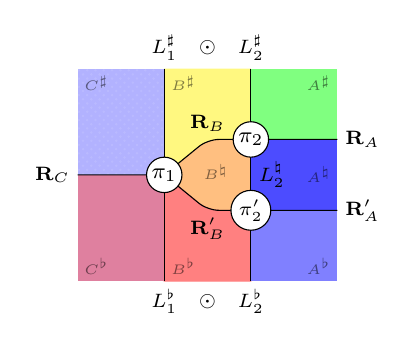
\begin{tikzpicture}[xscale=0.55,yscale=0.45,baseline=1.24cm]
      % Background
      % -- left band
      \fill[blue!30] (0,3) rectangle (2,6);
      \path[pattern color=white,pattern=crosshatch dots,opacity=0.1]
        (0,3) rectangle (2,6);
      \fill[purple!50] (0,0) rectangle (2,3);
      % -- center band
      \fill[yellow!50] (2,6) -- (2,3)
        [rounded corners] -- (3,4)
        [sharp corners] -- (4,4) |- cycle;
      \fill[orange!50] (4,4)
        [rounded corners] -- (3,4)
        [sharp corners] -- (2,3)
        [rounded corners] -- (3,2)
        [sharp corners] -| cycle;
      \fill[red!50,draw] (2,0) -- (2,3)
        [rounded corners] -- (3,2)
        [sharp corners] -- (4,2) |- cycle;
      % -- right band
      \fill[green!50] (4,4) rectangle (6,6);
      \fill[blue!70] (4,2) rectangle (6,4);
      \fill[blue!50] (4,0) rectangle (6,2);
      % Region labels
      \begin{scope}[opacity=0.5]
        \tiny
        \node[below right] at (0,6) {$C^\sharp$};
        \node[above right] at (0,0) {$C^\flat$};
        \node[below right] at (2,6) {$B^\sharp$};
        \node[yshift=1pt,xshift=3pt] at (3,3) {$B^\natural$};
        \node[above right] at (2,0) {$B^\flat$};
        \node[below left] at (6,6) {$A^\sharp$};
        \node[left] at (6,3) {$A^\natural$};
        \node[above left] at (6,0) {$A^\flat$};
      \end{scope}
      % Strings
      \begin{scope}
        \scriptsize
        \draw (0,3) node[left] {$\mathbf{R}_C$}
          -- (2,3) [rounded corners]
          -- (3,4) [sharp corners] node[above] {$\mathbf{R}_B$}
          -- (6,4) node[right] {$\mathbf{R}_A$};
        \draw (2,3) [rounded corners]
          -- (3,2) [sharp corners] node[below] {$\mathbf{R}_B'$}
          -- (6,2) node[right] {$\mathbf{R}_A'$};
        \draw (2,6) node[above] (L1s) {$L_1^\sharp$}
          -- (2,0) node[below] (L1f) {$L_1^\flat$};
        \draw (4,6) node[above] (L2s) {$L_2^\sharp$}
          -- node[right] {$L_2^\natural$}
          (4,0) node[below] (L2f) {$L_2^\flat$};
        \path (L1s) -- (L2s) node[midway] {$\odot$};
        \path (L1f) -- (L2f) node[midway] {$\odot$};
      \end{scope}
      % Nodes
      \begin{scope}[every node/.style={circle,draw,fill=white},inner sep=1pt]
        \footnotesize
        \node at (2,3) {$\pi_1$};
        \node at (4,4) {$\pi_2$};
        \node at (4,2) {\scriptsize $\pi_2'$};
      \end{scope}
    \end{tikzpicture}
  \]

  \vfill
  \[
      \pi_1 :
        L_1^\sharp
        \le_{\mathbf{R}_B \cdot \mathbf{R}_B' \twoheadrightarrow
             \mathbf{R}_C}
        L_1^\flat
      \qquad
      \pi_2 :
        L_2^\sharp
        \le_{\mathbf{R}_A \twoheadrightarrow \mathbf{R}_B}
        L_2^\natural
      \qquad
      \pi_2' :
        L_2^\natural
        \le_{\mathbf{R}_A' \twoheadrightarrow \mathbf{R}_B'}
        L_2^\flat
  \]

  \vfill
  \[
    \begin{prooftree}
      \hypo{\pi_1 \quad}
      \hypo{\pi_2 \quad}
      \hypo{\quad \pi_2'}
      \infer2{
	\pi_2 \odot \pi_2' \::\:
	L_2^\sharp
	\le_{\mathbf{R}_A \cdot \mathbf{R}_A' \twoheadrightarrow
	     \mathbf{R}_B \cdot \mathbf{R}_B'}
	L_2^\flat}
      \infer2{
	\pi_1 \otimes (\pi_2 \odot \pi_2')\: : \:
	L_1^\sharp \odot L_2^\sharp
	\le_{\mathbf{R}_A \cdot \mathbf{R}_A' \twoheadrightarrow
	     \mathbf{R}_C}
	L_1^\flat \odot L_2^\flat}
    \end{prooftree}
  \]

\end{frame}
%}}}

\begin{frame}{Contribution 2: Spatial composition} %{{{
  We introduce the tensor product of language interfaces
  \[
    A \otimes B = \langle A^\circ \times B^\circ, \, A^\bullet \times B^\bullet \rangle
  \]
  and investigate how it manifests in higher dimensions.

  \vfill
  \begin{center}
    \begin{tabular}{llclll}
      \toprule
      \multicolumn{6}{c}{\textbf{Spatial composition}} \\
      \midrule
      Object & & Dimension & \multicolumn{3}{c}{Operations} \\
      \midrule
      Language interface & $A$ & 1 & & & $\otimes$ \\
      Transition system & $L : A \twoheadrightarrow B$ & 2 & & $\odot$ & $\otimes$ \\
      Simulation convention & $\mathbb{R} : A \Leftrightarrow B$ & 2 & $\mathbin;$ & & $\otimes$ \\
      Simulation & $\rho : L_1 \le_{\mathbb{R} \twoheadrightarrow \mathbb{S}} L_2$ & 3 & $\mathbin;$ & $\odot$ & $\otimes$ \\
      \bottomrule
    \end{tabular}
  \end{center}
\end{frame}
%}}}

\begin{frame}{Contribution 3: Encapsulated state} %{{{
In order to account for objects,
we can add a new set $K$ of ``persistent states''
to transition systems,
and define them as
$\langle S, K, {\rightarrow}, I, X, Y, F \rangle$ where
\begin{itemize}
  \item $I \subseteq K \times B^\que \times S$
  \item $F \subseteq S \times B^\ans \times K$
\end{itemize}

\vfill
But that is the same as using the incoming language interface $B \otimes [K]$:
\begin{itemize}
  \item $I \subseteq (K \times B^\que) \times S$
  \item $F \subseteq S \times (B^\ans \times K)$
\end{itemize}

\vfill
In fact, our theory of spatial composition
gives tools for plumbing state.

We use it to build a model with
encapsulation and representation independence.
\end{frame}
%}}}
  

\begin{frame}{Plan} %{{{
\begin{description}
  \item[4/14] OOPSLA submission deadline
    \begin{itemize}
      \item make paper more accessible
      \item document the full example
      \item complete artifact
    \end{itemize}
  \item[after] New CompCertO framework
    \begin{itemize}
      \item External to CompCert
      \item Support effect signatures
    \end{itemize}
  \item[after] RBGS trace semantics / refinement conventions
    \begin{itemize}
      \item need to fix and understand the math better
    \end{itemize}
\end{description}
\end{frame}
%}}}

\section{Composition in CompCert} %{{{

\begin{frame}{Semantics in CompCertO} %{{{
  CompCertO transition systems can interact through \emph{language interfaces},
  where \\ a language interface $A = \langle A^\circ, A^\bullet \rangle$
  is a set of \emph{questions} $q \in A^\circ$
  and \emph{answers} $r \in A^\bullet$.

  \vfill
  $L : A \twoheadrightarrow B$
  handles an incoming call in $B$ and
  may perform outgoing calls in $A$.

  \vfill
  \begin{columns}
    \begin{column}{0.55\textwidth}
      It is given as $L = \langle S, {\rightarrow}, I, X, Y, F \rangle$ where
      \\ in particular:
      \begin{itemize}
      %  \item $S$ is a set of states
      %  \item ${\rightarrow} \subseteq S \times S$ is a transition relation
        \item $I \subseteq B^\circ \times S$ gives initial states;
        \item $F \subseteq S \times B^\bullet$ gives final states;
        \item $X \subseteq S \times A^\circ$ identifies external states and
        \item $Y \subseteq S \times A^\bullet \times S$ resumption states.
      \end{itemize}
    \end{column}
    \begin{column}{0.35\textwidth}
        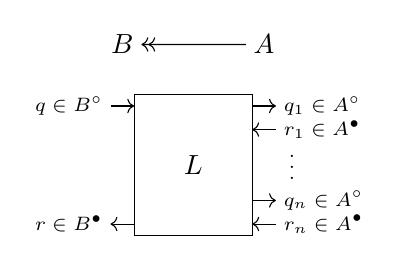
\begin{tikzpicture}[yscale=0.15,xscale=0.30]
          \draw (0,-1) rectangle (5,11) node[midway] {$L$};
          \scriptsize
          \draw[->] (-1,10) node[left] {$q \in B^\que$} -- (0,10)
              node[above=2em,midway] (B) {\normalsize $B$};
            \draw[->] (5,10) -- (6,10) node[right] {$q_1 \in A^\que$}
              node[above=2em,midway] (A) {\normalsize $A$};
            \draw[->] (6,8) node[right] {$r_1 \in A^\ans$} -- (5,8) ;
            \node[right] at (6,5.5) {$\:\vdots$};
            \draw[->] (5,2) -- (6,2) node[right] {$q_n \in A^\que$};
            \draw[->] (6,0) node[right] {$r_n \in A^\ans$} -- (5,0);
          \draw[->] (0,0) -- (-1,0) node[left] {$r \in B^\ans$};
          \draw[->>] (A) -- (B);
        \end{tikzpicture}
    \end{column}
  \end{columns}

  \vfill
  %For example:
  \[
    q \mathrel{I} s_0 \rightarrow s_1 \mathrel{X} q_1 \leadsto r_1 \mathrel{Y^{s_1}} s_2
                      \rightarrow \cdots
                      \rightarrow s_3 \mathrel{X} q_n \leadsto r_n \mathrel{Y^{s_1}} s_4
                      \rightarrow s_5 \mathrel{F} r
  \]
\end{frame}
%}}}

\begin{frame}{Composing Transition Systems \fbox{$\odot$}}
\end{frame}

%}}}

\section{Persistent state} %{{{

\begin{frame}{State in CompCertO} %{{{
  In the C language modeled by CompCert,
  all state is either:
  \begin{itemize}
    \item local to a particular \emph{activation}
      (temporaries stored in a local environment);
    \item stored in the global memory
      (incl. stack-allocated variable).
  \end{itemize}
  Therefore,
  in Compositional CompCert and CompCertO
  there is no need for local state
  to surivive a particular activation.

  \vfill
  By contrast,
  objects, closures, abstraction layers
  all maintain state across successive activations:
  \begin{itemize}
    \item behavior is history-sensitive, but
    \item the state cannot be observed directly by the environment.
  \end{itemize}

  \vfill
  \begin{columns}
    \begin{column}{0.55\textwidth}
      It is given as $L = \langle S, {\rightarrow}, I, X, Y, F \rangle$ where
      \\ in particular:
      \begin{itemize}
      %  \item $S$ is a set of states
      %  \item ${\rightarrow} \subseteq S \times S$ is a transition relation
        \item $I \subseteq B^\circ \times S$ gives initial states;
        \item $F \subseteq S \times B^\bullet$ gives final states;
        \item $X \subseteq S \times A^\circ$ identifies external states and
        \item $Y \subseteq S \times A^\bullet \times S$ resumption states.
      \end{itemize}
    \end{column}
    \begin{column}{0.35\textwidth}
        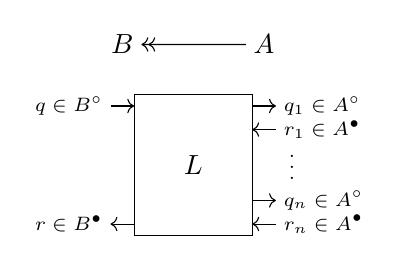
\begin{tikzpicture}[yscale=0.15,xscale=0.30]
          \draw (0,-1) rectangle (5,11) node[midway] {$L$};
          \scriptsize
          \draw[->] (-1,10) node[left] {$q \in B^\que$} -- (0,10)
              node[above=2em,midway] (B) {\normalsize $B$};
            \draw[->] (5,10) -- (6,10) node[right] {$q_1 \in A^\que$}
              node[above=2em,midway] (A) {\normalsize $A$};
            \draw[->] (6,8) node[right] {$r_1 \in A^\ans$} -- (5,8) ;
            \node[right] at (6,5.5) {$\:\vdots$};
            \draw[->] (5,2) -- (6,2) node[right] {$q_n \in A^\que$};
            \draw[->] (6,0) node[right] {$r_n \in A^\ans$} -- (5,0);
          \draw[->] (0,0) -- (-1,0) node[left] {$r \in B^\ans$};
          \draw[->>] (A) -- (B);
        \end{tikzpicture}
    \end{column}
  \end{columns}

  \vfill
  %For example:
  \[
    q \mathrel{I} s_0 \rightarrow s_1 \mathrel{X} q_1 \leadsto r_1 \mathrel{Y^{s_1}} s_2
                      \rightarrow \cdots
                      \rightarrow s_3 \mathrel{X} q_n \leadsto r_n \mathrel{Y^{s_1}} s_4
                      \rightarrow s_5 \mathrel{F} r
  \]
\end{frame}
%}}}

%}}}

\end{document}
